\input{chapter-header.tex}
% ===========================================================================
\part{State of the Art}
\chaplabel{background}
\minitoc
% ===========================================================================

%Software inevitable changes and we need to provide with the tools and methodologies that support such changes~\cite{Nier08b}. However, production-ready applications are not usually change-aware. These applications should be either engineered from scratch with change in mind, or a lot of reengineering effort should be invested in them to support change. Making deep modifications to a language runtime can be a cumbersome task.

This chapter presents the related work to this dissertation. With that in mind, we organize and classify the related work in two different axis. We will first explore work that is related to this dissertation on its objective: runtime manipulation. Afterwards we will give an overview on virtualization related technique that inspired our work. The reader would notice that some of the related works we present may fit into both these categories, according to our point of view. However, for the sake of clarity, we emphasize the aspects we believe will clarify the understanding of the rest of this thesis.

The first part of this chapter focuses on runtime manipulation of object-oriented applications. We first show the problems that arise in state of the art languages when trying change their runtime representation. Then we go inside the related work that focus on the safe modification of language semantics at runtime. Then, we show how metacircular runtimes aim to have an unified language runtime to ease its modification. \gp{conclusion?}

The second part of this chapter starts by presenting a brief introduction to virtualization, its terminology and moreover its usage. We continue by identifying virtualization-related techniques applied to the manipulation of language runtimes in the state of the art.  \gp{conclusion?} 

This chapter finishes by presenting a detailed description of the problem statement and a final outlook of the upcoming chapters in the light of the found problems.


% ===========================================================================
\newpage
% ===========================================================================

\chapter{Modifying the Runtime}

In the following sections we present related work that aim to modify a language runtime, sorted in two main categories. First, we present related work that targets the modification of a language's semantics at runtime by safe means~(\ie avoiding crashes). We follow by looking at the field of metacircular runtimes and \VMs, to study how they ease the modification of a runtime by means of simplifying the language-\VM relation for development.

\section{Modification of language semantics}

\subsection{\textsc{Tower of Interpreters Model}}

The original model of reflection as defined by Smith~\cite{Smit82c} is based on meta-level interpretation. A program is interpreted by an interpreter, such interpreter is interpreted by a meta-interpreter and so on, possibly ad-infinitum. This leads to a tower of interpreters, where each floor defines the semantics of the program~(interpreter of application) it interprets~(Figure \ref{fig:tower_of_interpreters}).

\begin{figure}[ht]
\begin{center}
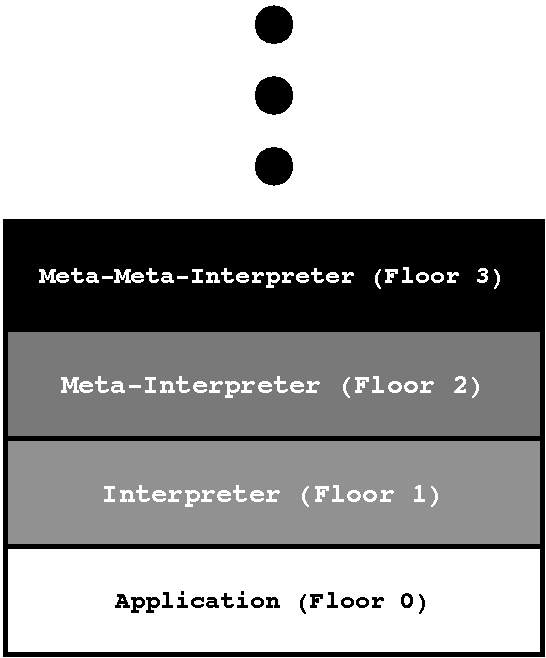
\includegraphics[width=.5\linewidth]{tower_of_interpreters}
\caption{\textbf{The theoretical tower of interpreters model.} Each floor interprets the floor below itself.\label{fig:tower_of_interpreters}
% (a)The host language and (b)the guest language contain each one their own classes and objects. The guest language resides inside the host language during the bootstrap; (c)the builder, a program written in the host language, reifies the bootstrap process itself and bootstraps the guest language given a (d)source code specification.
 }
\end{center}
\end{figure}

The tower of interpreters presents a model where one can define and redefine the semantics of the program it is executing. We can modify the behavior of our program~(in the floor zero) by jumping one level above it in the tower and modifying the interpreter running in that floor. In the same sense, we can jump one level above this interpreter to change also its behavior and so on. This allows the \emph{indirect modification} of a program's behavior \ie a change in an interpreter in a level \emph{n} changes the behavior of the interpreter level \emph{n - 1}, which impacts in the interpreter below it and so on, up to the base level.

Smith's tower of interpreters model is flexible and coherent regarding the manipulation of the reflective behavior of a program. The tower does not present a limit on the amount of interpreters we can stack, presenting a problematic infinite potential. This idea collides with the non-infinite amount resources in current hardware. On one side, limited memory prevents us to have a tower of infinite interpreters running at the same time. On the other side, above certain limit of interpreters, this approach becomes too slow and impractical. We will show in the following subsections other reflective models that try to overcome these deficiencies while trying to keep some of the good properties of this model.

\subsection{\textsc{Black}}

Black is a reflective language based on Scheme that mimics the infinite tower of interpreters with the goal to make it practical. Its model is based on the same idea as the reflective tower: the base level is interpreted by an interpreter, which is interpreted by a meta-interpreter and so on. The main difference between the original tower of interpreters and the model presented by Black is that the latter avoids the infinite regression, making the model practical in finite resource machines.

Black avoids the infinite regression by limiting the real levels of interpretation: there is only one level of interpretation. For the rest of the levels, Black  introduces a difference between directly-executed code in contrast with interpreted code. Directly-executed code is code that is executed by the machine, where no interpretation steps are involved. Then, the base-level application is the only interpreted code in the application. The rest of the tower, including the first interpreter, is implemented and executed directly in machine code~(Figure \ref{fig:black_tower}).

\begin{figure}[ht]
\begin{center}
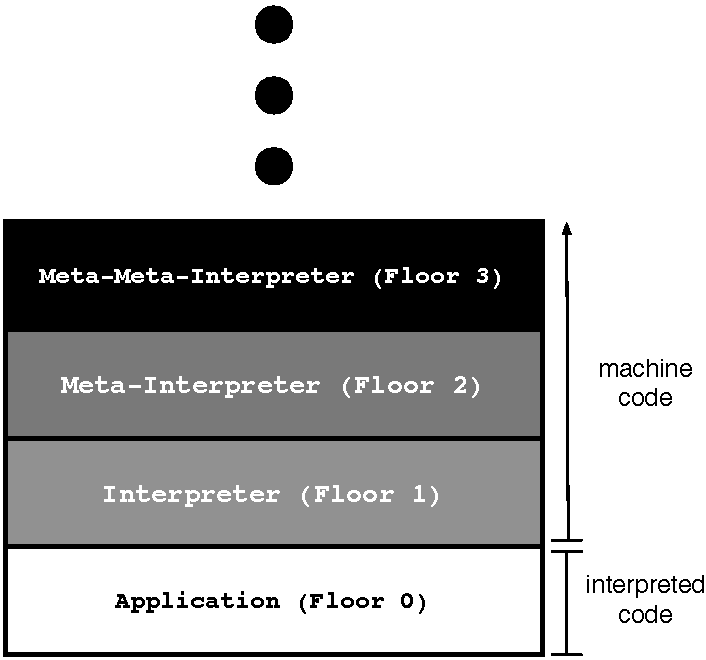
\includegraphics[width=.6\linewidth]{black_tower}
\caption{\textbf{Black model of interpreters.} Only the application level is interpreted. The levels above are directly executed on the machine.\label{fig:black_tower}
% (a)The host language and (b)the guest language contain each one their own classes and objects. The guest language resides inside the host language during the bootstrap; (c)the builder, a program written in the host language, reifies the bootstrap process itself and bootstraps the guest language given a (d)source code specification.
 }
\end{center}
\end{figure}

By limiting the levels of interpretation, the model presented by Black forbids \emph{indirect modification}. Changing the interpreter in a level \emph{n} above the first level does not impact any more the interpreters below it, as they are directly-executed in the machine and not by the modified interpreter. Black supports, however, the modification of the first level of interpretation with the introduction of hooks inside the machine code. A hook detects wether a function in the interpreter~(written in directly-executed code) is changed, and interprets it by a meta-level interpreter written also in directly executed code. Hooks degrade the performance in comparison of a non-hooked interpreter, but it allows in exchange to change and specialize the behavior of the directly-executed code.

\subsection{\textsc{Safe-Tcl}}
Safe-Tcl~\cite{Levy97a, Bore94a} is a variation of Tcl whose main purpose is the execution of Tcl scripts in a safe environment, with restricted permissions and attributions. Safe-Tcl achieves this by using \emph{twin interpreters} \ie a normal Tcl interpreter~(the master interpreter) can invoke another interpreter and specialize its behavior. Both the master child interpreters run isolated from each other~(Figure \ref{fig:safetcl_twin_interpreters}).

\begin{figure}[ht]
\begin{center}
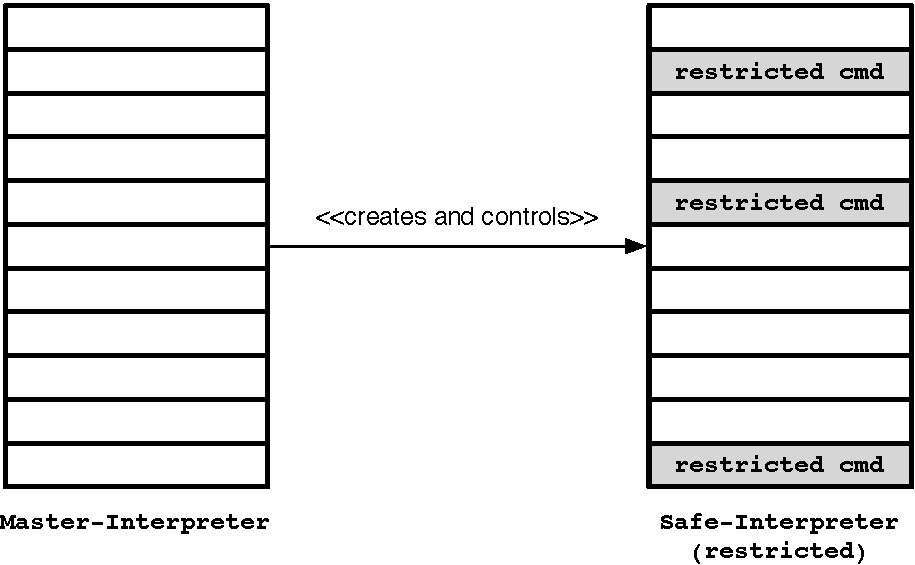
\includegraphics[width=.6\linewidth]{safetcl_twin_interpreters}
\caption{\textbf{SafeTcl Twin Interpretation.} The Master interpreter creates and configures a safe interpreter. The safe interpreter, with modified commands, will run the sandboxed Tcl application.\label{fig:safetcl_twin_interpreters}
% (a)The host language and (b)the guest language contain each one their own classes and objects. The guest language resides inside the host language during the bootstrap; (c)the builder, a program written in the host language, reifies the bootstrap process itself and bootstraps the guest language given a (d)source code specification.
 }
\end{center}
\end{figure}

The master interpreter modifies the behavior of a safe interpreter by providing a security policy. A security policy grants or removes privileges to the scripts executed on an interpreter. Commands can be aliased so the untrusted interpreter call an aliased method and the command is fully implemented by a trusted interpreter.

Safe-Tcl twin interpretation allows us to change the behavior of a program running on a specialized interpreter, without the limitations of the infinite tower of interpreters. However, in contrast with the solutions we already presented, Safe-Tcl does not provide with the ability to change completely the semantics of the language but just to override or provide new commands, with a focus on security.

\subsection{\textsc{Reflectivity: scoping reflection in Reflective Architectures}}

To enable reflection in mainstream languages such as Java, Ruby or JavaScript, the tower of interpreters is replaced by a reflective architecture~\cite{Maes87a}. Instead of relying on a stack of interpreters interpreting each the level below it, a reflective architecture relies on the idea of \emph{causal connection} \ie the programming language incorporates structures that represents aspects of itself~(\eg classes, objects), in such a way that if one structure changes the aspect it represents is updated accordingly, and vice-versa.


In languages presenting reflective architectures, reflection is controlled by meta-objects that live in the same environment of the object it reflects upon.
One problematic corollary of this is that meta-objects rely on the same code and infrastructure than the objects they reflect upon; therefore there is a risk of infinite meta-recursion when the meta-level instruments code that it relies upon~(Figure \ref{fig:reflectivity_meta_recursion}).

\begin{figure}[ht]
\begin{center}
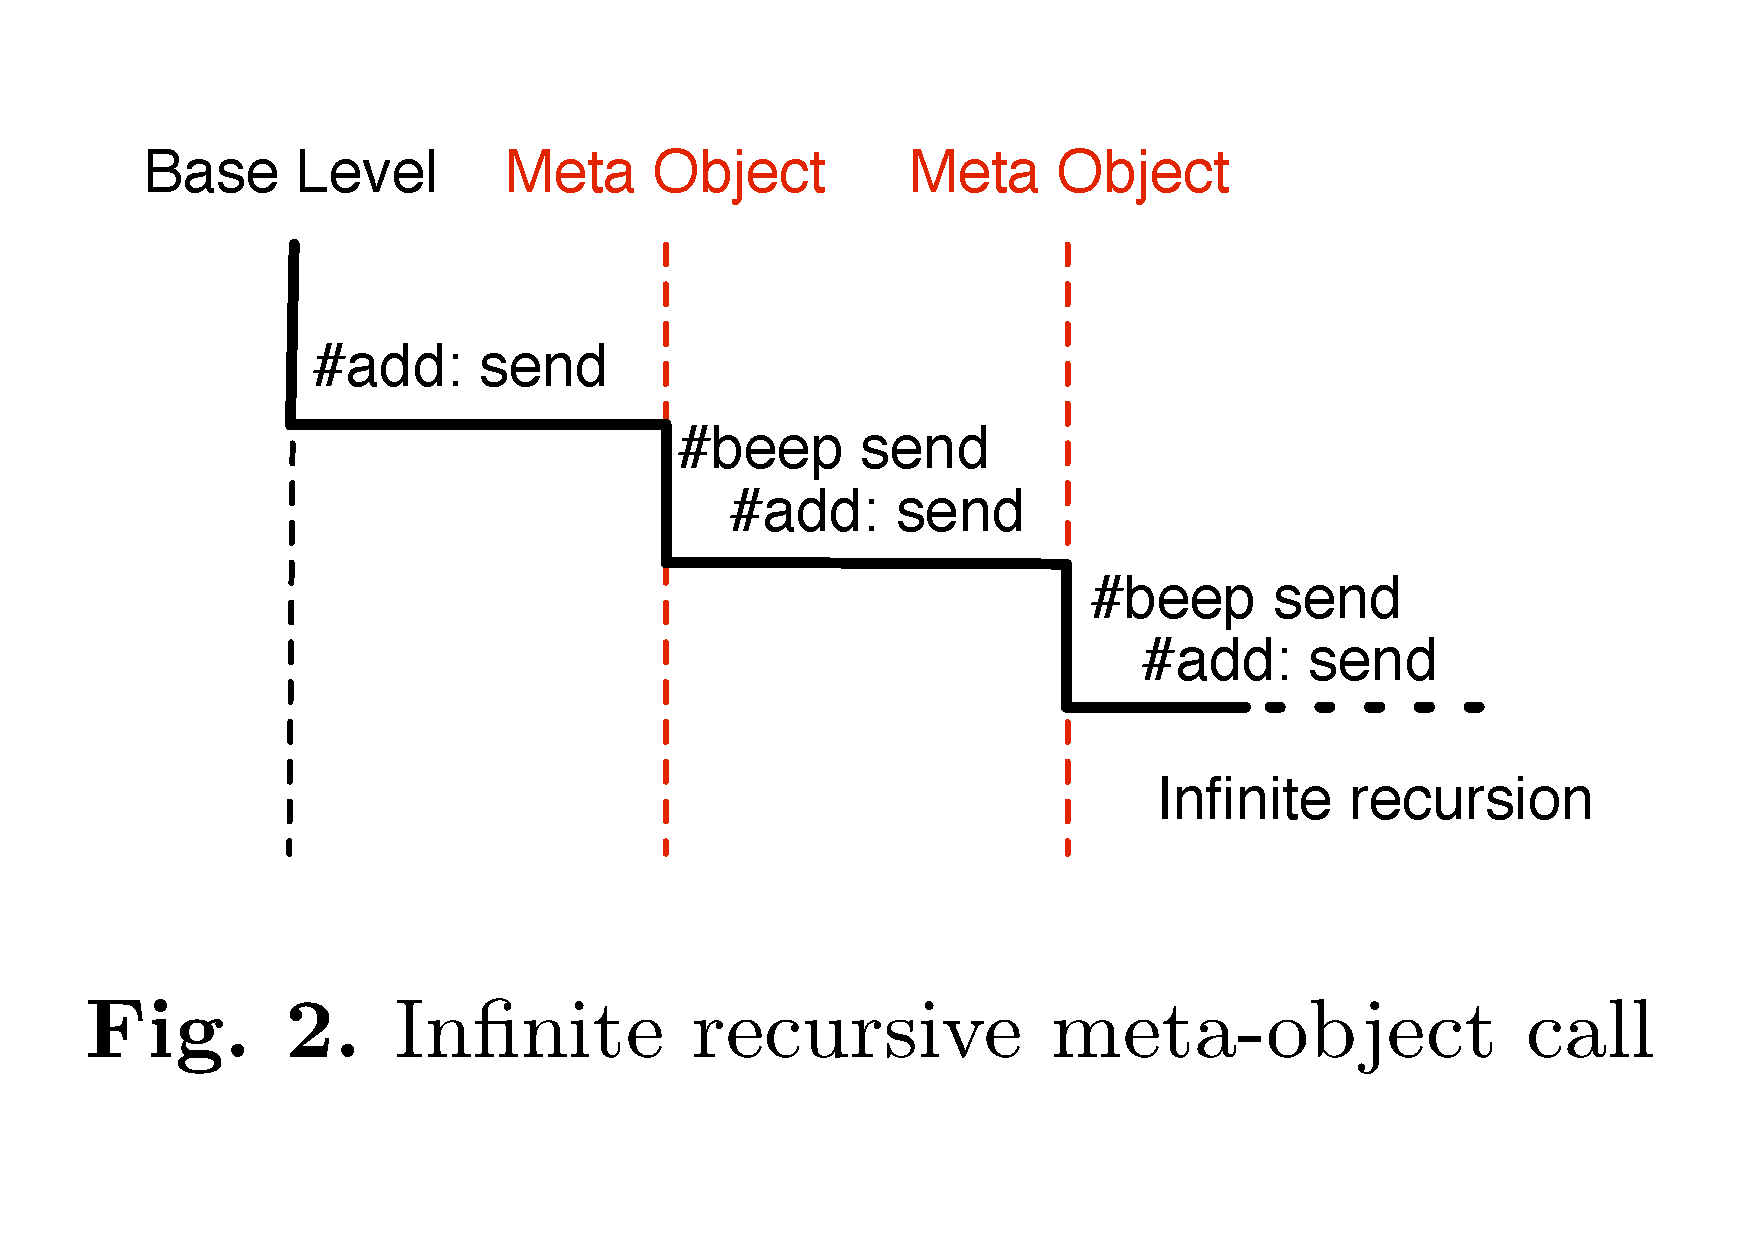
\includegraphics[width=.6\linewidth]{reflectivity_meta_recursion}
\caption{\textbf{Meta level recursion in reflective architectures.}\label{fig:reflectivity_meta_recursion}
% (a)The host language and (b)the guest language contain each one their own classes and objects. The guest language resides inside the host language during the bootstrap; (c)the builder, a program written in the host language, reifies the bootstrap process itself and bootstraps the guest language given a (d)source code specification.
 }
\end{center}
\end{figure}

Denker et al. solve this problem in Reflectivity~\cite{Denk08b}. Reflectivity is a reflective framework that avoids meta-recursions by tracking the degree of metaness of the execution context. In each reflective call, the \ct{MetaContext} object is activated and it accounts the meta-level jump. Likewise, when the reflective call returns, the \ct{MetaContext} is deactivated. Using the accounted meta-level jumps of the \ct{MetaContext}, meta-objects do only reflect on objects of a lower metaness~(and not greater or equal metaness). Thus, it simulates the semantics of an infinite tower of distinct interpreters while there is only one of them~(Figure \ref{fig:reflectivity_avoid_meta_recursion}).

\begin{figure}[ht]
\begin{center}
\begin{subfigure}{.45\textwidth}
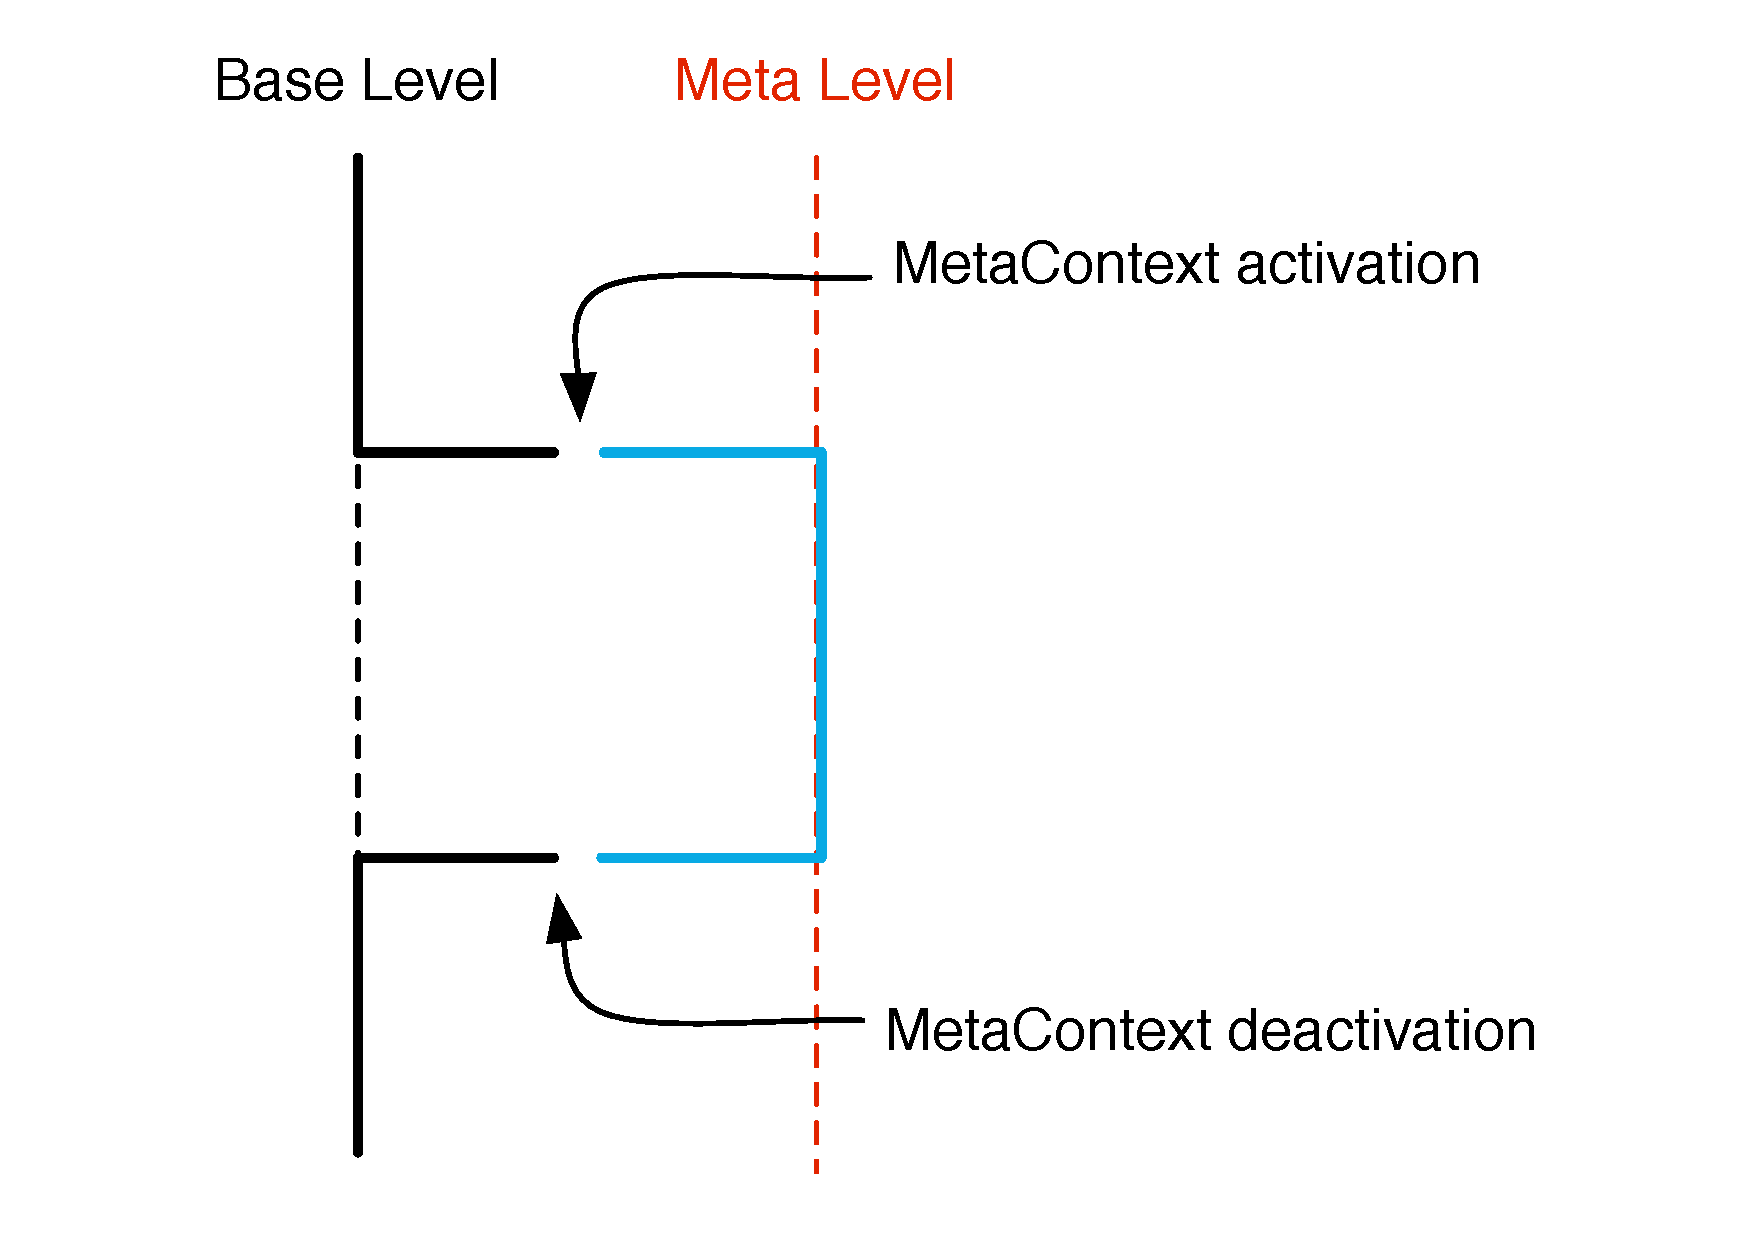
\includegraphics[width=1\linewidth]{reflectivity_metaness_accounting}
\end{subfigure}
\begin{subfigure}{.45\textwidth}
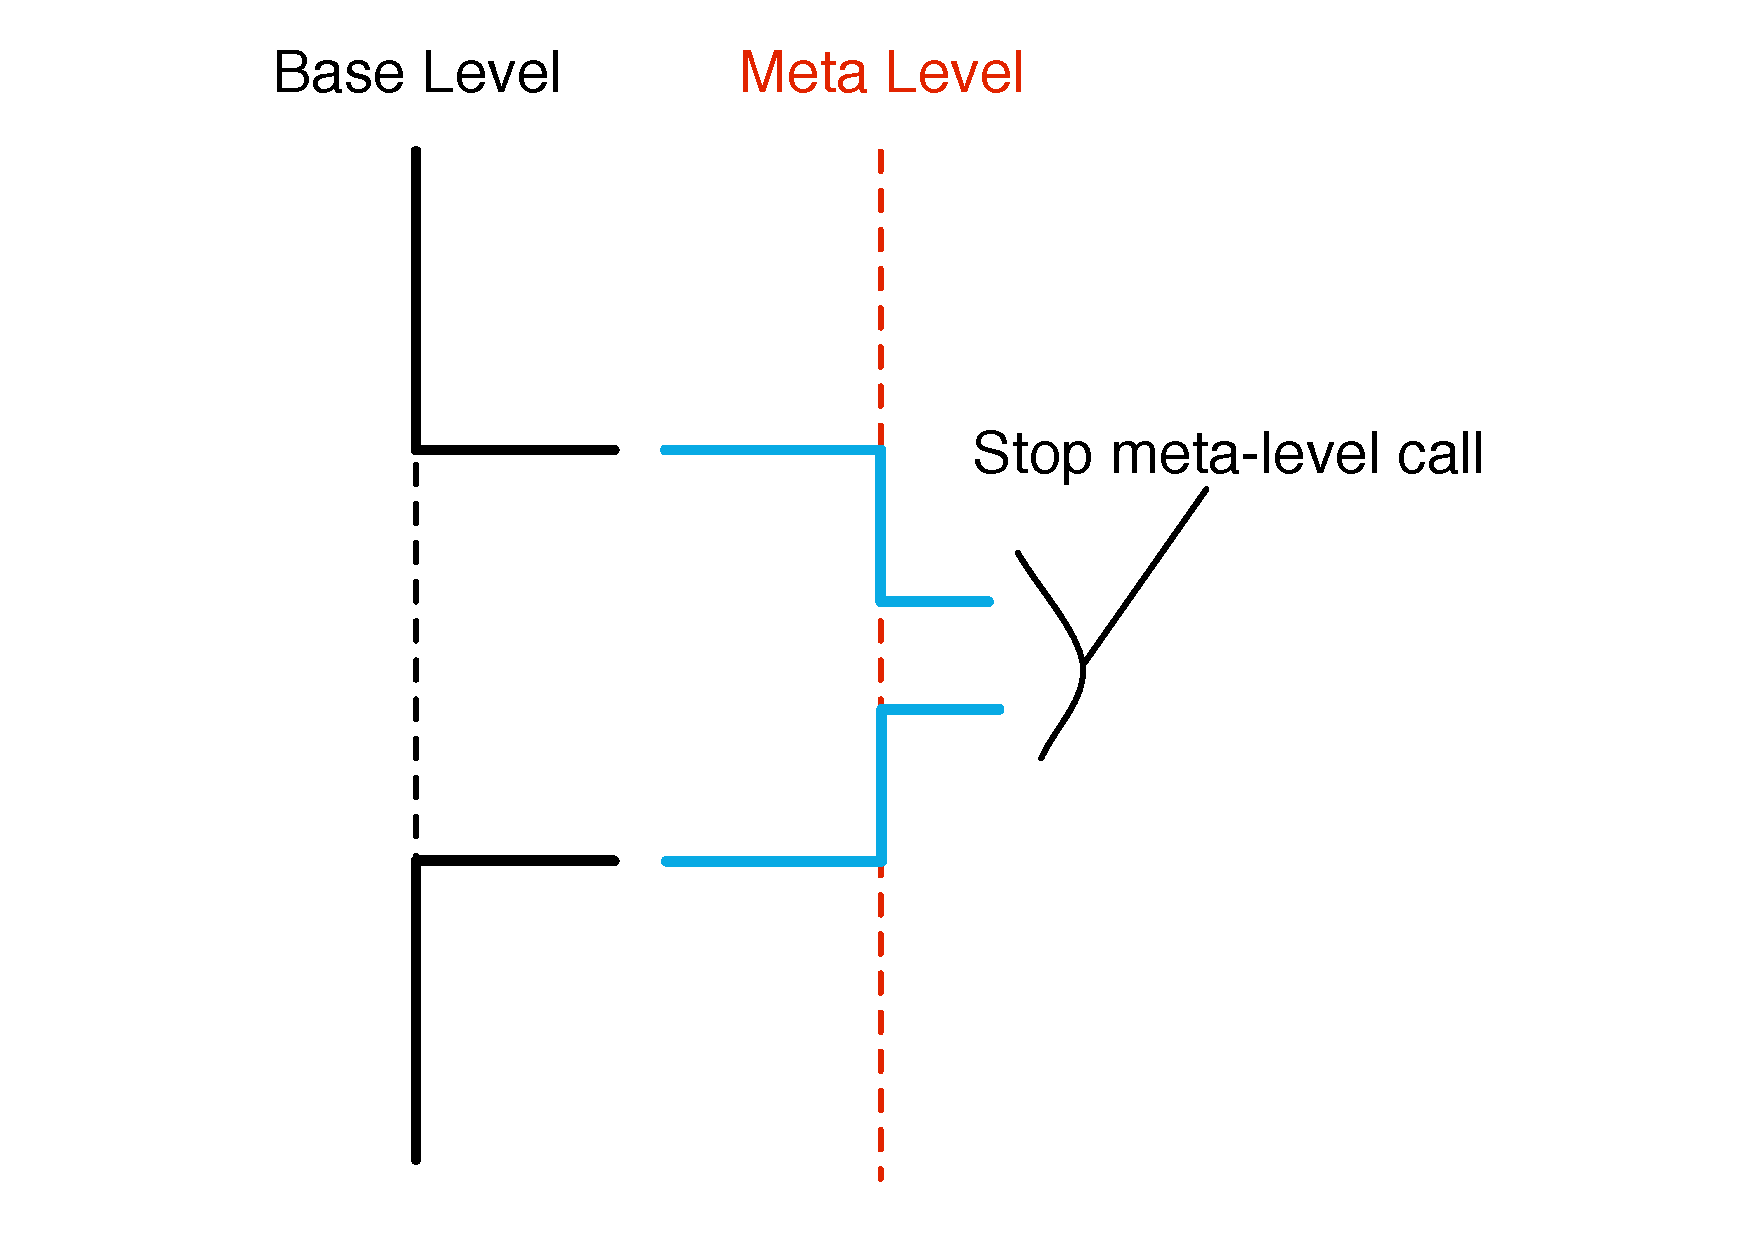
\includegraphics[width=1\linewidth]{reflectivity_avoid_recursion}
\end{subfigure}
\caption{\textbf{Meta level jump using reflectivity.}\label{fig:reflectivity_avoid_meta_recursion}
% (a)The host language and (b)the guest language contain each one their own classes and objects. The guest language resides inside the host language during the bootstrap; (c)the builder, a program written in the host language, reifies the bootstrap process itself and bootstraps the guest language given a (d)source code specification.
 }
\end{center}
\end{figure}

Reflectivity succeeds to modify and scope behavioral reflection for different meta-levels inside the same reflective architecture. However, it does not provide with support to fully change the language semantics~(residing in the \VM) or to perform structural reflection.

\section{Metacircular Runtimes}

High-level language \VMs are inherent complex pieces of software.
They have to combine two rather extreme goals: abstraction and performance.
We have seen that the required abstraction for the running high-level language has a strong influence on the \VM design.
At the same time the hard performance requirement requires precise interaction with the underlying hardware.
This goes even so far that specialized hardware is conceived to match the performance requirements~\cite{Unga84a,Stef84a,McGh98a,Clic05a}.

The early \VMs focused on interpreting an abstract instruction set (bytecodes).
The benefits are twofold.
On the one hand the bytecodes guarantee certain platform independence by abstracting away from the \CPU specific instruction set.
On the other hand bytecodes allow to encode complex operations into little space both serving the hard memory constraints of the hardware and simplifying the design of a compiler.
Obviously this abstraction gain comes at a cost and ever since the first \VMs were built research and industry strive to reduce the interpretation overhead.
An efficient way to improve performance is to use a just in time compiler (JIT) that dynamically generates native code from the bytecode~\cite{Deut84a}.
In this case the bytecode becomes an intermediate representation (IR) for a bigger compiler infrastructure.
However, JIT compilers are notoriously complex as they crosscut many \VM components.
At the same time they crosscut all abstraction layers; they have to access high-level information from the running bytecodes and manage native code at the same time.
Similar complexity applies to the automatic memory management present in most high-level language \VMs.
Garbage Collectors (GC) evolved from simple helpers to complex software artifacts that for instance support concurrent garbage collection~\cite{Clic05a}.
Moreover, this complexity impacts the language running on top of these \VMs. The unclear interface between the language and the VM makes difficult to recognize whether a piece of code belongs to a VM or language concern.

The increased complexity of the \VMs lead to more novel approaches on how to build \VMs.
\VMs are still build for a big part in C or C++ for performance reasons.
However, there are more high-level approaches that try to simplify creating \VMs by using building blocks~\cite{Geof10a}.
In the following sections we are shedding light on metacircular \VMs which are programmed in the same language they in the end support.


\subsection{\textsc{Squeak Smalltalk \VM}}
\seclabel{background-squeak}
% ---------------------------------------------------------------------------
The Squeak \VM~\cite{Inga97a} is of importance in the context of this work.
Its core building system is still in active use for the \urlfootnote{Cog \VM}{http://www.mirandabanda.org/cogblog/} which extends Squeak with a JIT compiler.
The Cog \VM is used as default by the \urlfootnote{Pharo}{http://pharo.org/} programming language.
The Squeak \VM is built around a Smalltalk dialect called Slang that is exported to C to be compiled to the final \VM binary.
Additionally, the Slang sources can be interpreted to provide an interactive simulator of the \VM, including full graphical support.

Slang is limited to the functionality that can be expressed with standard C code.
Slang in this case is mostly a high-level C preprocessor.
Even though Slang basically has the same syntax as Smalltalk it is semantically constrained to expressions that can be resolved statically at compilation or code generation time and are compatible with C.
Hence Slang's semantics are closer to C's than to Smalltalk's.
Unlike later metacircular frameworks, Squeak uses little or no compile-time reflection to simplify the \VM designs.
However, class composition help structuring the sources.
Next to the Slang source which account for the biggest part of the interpreter code some operating system related code and plugins are written in C.
To facilitate the interaction with the pure C part Slang supports inline C expressions and type annotations.

A great achievement of the Squeak \VM is a simulator environment that enables programmers to interact dynamically with the running \VM sources.
The simulator is capable or running a complete Squeak Smalltalk image including graphical user interface.
This means that programmers can change the sources of the running \VM and see the immediate effects in the simulator.
The simulator itself works by setting up a byte array which servers as native memory.
Then the \VM sources written in Slang are interpreted by the \VM of the development environment.

% ---------------------------------------------------------------------------
\subsection{\textsc{Jikes: High-level low-level Programming with MMTK}}
\seclabel{background-jikes}
% ---------------------------------------------------------------------------
Jikes (former Jalapeño) is an early metacircular research \VM for Java written in Java~\cite{Alpe00a}.
The Jikes \VM features several different garbage collectors and does not execute bytecodes but directly compiles to native code.
With metacircularity in mind Jikes does not resort to a low-level programming language such as C for these typically low-level \VM components.
Instead they are written in Java as well using a high-level low-level programming framework.

The Jikes \VM had performance as a major goal, hence direct unobstructed interaction with the low-level world is necessary using a specialized framework.
High-level low-level programming \cite{Fram09a} is mentioned the first time in the context of the Jikes \VM project.
The goal of high-level low-level programming is to provide high-level abstractions to simplify low-level programming.
Essentially this is the same motivation that drives the metacircular \VM community.

Frampton et al. present a high-level low-level framework packaged as \ttt{org.vmmagic}, which is used as a system interface for Jikes. This package introduces highly controlled low-level interaction in a statically type context.
In their framework, methods have to be annotated to enable the use of low-level functionality.
Additionally their framework is successfully used in a separate project, the memory management toolkit (\textsc{MMTK})~\cite{Blac04a} which is used independently in several other projects.


% ---------------------------------------------------------------------------
\subsection{\textsc{Maxine Java \VM}}
\seclabel{background-maxine}
% ---------------------------------------------------------------------------
Maxine is a metacircular Java \VM~\cite{Wimm13a} focused on an efficient developer experience.
Typically \VM frameworks focus on abstraction at the code-level which should yield simpler code and thus help reducing development efforts.
However, in most situations the programmer is still forced to use existing unspecific tools for instance to debug the \VM.
In contrast to that, the Maxine \VM provides dedicated tools to interact with the \VM in development.
Maxine uses abstract and high-level representations of \VM-level concepts and consistently exposes them throughout the development process.
Inspectors at multiple abstraction levels are readily available while debugging, giving insights to the complete \VM state.
Maxine provides and excellent navigation for generated native code by providing links back to language-side objects as well as other native code and symbols.

Even though the Maxine projects follows an approach where reflection is only used at compile-time, the development tools themselves provide a live interaction with the running \VM artifact.
However, the \VM itself is not reflective as it is not directly built to reason about itself.
This means that when debugging the \VM it behaves almost like a living Smalltalk image where a complete interaction with the underlying system is possible.
We identify this as crucial, as most of the time is spent debugging, notably on inadequate tools like \ttt{gdb} due to lack of alternatives.
Hence having a specific debuggers and inspectors greatly improve the interaction with the \VM artifact.


\subsection{\textsc{PyPy Toolchain}}
\seclabel{background-pypy}
% ---------------------------------------------------------------------------
\urlfootnote{PyPy}{http://pypy.org/} is a Python-based high-level \VM framework~\cite{Rigo06a}.
PyPy's major focus lies on an efficient Python interpreter.
However, it has been successfully used to build \VMs for other languages including Smalltalk~\cite{Bolz08a}.
Interpreters are written in a type-inferable subset of Python called RPython.
The underlying PyPy infrastructure automatically provides memory management and JIT compilation.
Instead of explicitly providing these features, a \VM developer hints certain information to the PyPy framework to improve the generation of a GC or JIT.

PyPy follows a different approach from the previously presented \VM generation frameworks.
For instance, in Squeak and Jikes the final \VM implementation is not much different from an implementation done directly in a low-level language.
The programmer specifies all the components of the \VM explicitly, either by implementing them directly or using a provided library.
Compared to the more static C and C++ these \VM generation frameworks make the compilation phase more tangible.
Smalltalk in Squeak or Java in Jikes or Maxine fulfill the purpose of the template system in C++ or the restricted macro system in C.
For the explicit implementation part PyPy is no different.
However, certain features for the final \VM are directly absorbed from the underlying PyPy infrastructure.
For instance, the JIT support or the GC are not explicitly implemented but provided by the PyPy framework itself.
This is a big difference to the other \VM frameworks as it allows programmers to write the \VM in a more high-level fashion.
For instance in Squeak memory allocation, even for \VM-level objects, has to be performed explicitly.
Whereas in PyPy the garbage collection is left to the underlying \VM building infrastructure.
This approach allows RPython \VMs to behave like standard Python programs.

Much like the automatic memory management, PyPy provides a tracing JIT generator~\cite{Bolz09a}.
By default the \VM programmer does not write an explicit JIT in PyPy.
Instead the \VM code is annotated to guide the underlying tracing JIT generator.
This means a \VM compilation time a specific tracing JIT is created for the given meta information.
As a result, the JIT can track high-level loops in the final interpreted language.
Again, this is similar to PyPy's GC, both are provided as a service and do not have to be programmed explicitly.
Instead, the \VM programmer tweaks parameters of the JIT or GC.

% ------------------------------------------------------------------------------
\subsection{\textsc{Pinocchio \VM}}
\seclabel{background-Pinocchio }

Pinocchio~\cite{Verw11a} is a research Smalltalk environment that directly uses native code instead of bytecodes.
The only execution base is native code which is directly generated by the language-side compiler.

Pinocchio is built from a kernel derived originally from a \PH image.
For the bootstrap classes, objects and methods are exported into binary, native images and linked together with a standard C linker to a final executable.
For simplicity it relies on a very small part of C code to provide essential primitives, for instance used for file handling.
Additionally it specifies part of the bootstrap for the Smalltalk object model in plain C code.
However, besides that, all the other code is written and developed directly in Smalltalk.

An important aspect of Pinocchio is that the method lookup is expressed in terms of normal Smalltalk code.
Typically this code statically resides in the \VM, thus at a different meta-level.
Hence this implies for most systems that the lookup can not be modified without altering the \VM itself.
However, expressing the lookup in terms for normal language-side code introduces a recursive dependency during the bootstrap.
In order to run the lookup code expressed in Smalltalk code, we have to perform message sends.
These, in return, require an already working lookup mechanism.
Hence, without taking special care, a language-side lookup method will lead to infinite recursion during startup.
Pinocchio resolves this problem by directly interacting with the low-level execution format which among other things relies on inline caches to improve performance.
The important property of inline caches is that they bypass the slow language-side lookup by directly jumping to the last activated method at a send-site.
This is exactly the behavior we need to prevent recursion during the startup.
Hence, when generating the native code for the bootstrap, it prefills all the inline caches of the methods required to perform a full method lookup.
As a result, when at runtime it is required the first real method lookup, the lookup code itself is running perfectly on the prefilled inline caches.
Pinocchio achieves a flexible connection between the low-level world and the high-level language-side.
During execution, the \VM jumps freely between what previously was native \VM-level code and interpretation of language-side code.

% ------------------------------------------------------------------------------
\subsection{\textsc{Klein \VM}}
\seclabel{background-klein}

\urlfootnote{Klein}{http://kleinvm.sourceforge.net/} is a metacircular \VM for the Self programming language that has no separation into \VM and language \cite{Unga05a}.
It is important to point out that the reification of the \VM-level survives the code generation or compilation time.
Instead the \VM structures are represented as real Self objects.
Hence the Klein \VM supports true \VM-level reflection since there is only a single code base.

Additionally to the advances in reflection and metacircularity, Klein focuses on fast compilation turnarounds to allow for a responsive development process.
Which is unlike for instance the Squeak \VM where a full \VM bootstrap takes an order of minutes on modern hardware.
Klein also supports advanced mirror-based debugging tools to inspect and modify a remote \VM.

Development on the Klein \VM stopped in 2009 and left the Klein \VM in fairly usable state.
Yet, it proved that it is possible and build a language-runtime without the classical separation of the language-side and the \VM.
From the literature presented about the Klein project we see a strong focus on the improvements of the development tools.
The fact that the language-runtime allows \VM-level reflection to change the \VM dynamically is not directly mentioned in the literature.
While we see the practical limitations of changing the \VM runtime system at runtime we would like to open the doors to this new form of reflection.

\chapter{Specializing Applications for Memory Footprint}

The reduction of the deployment footprint of object-oriented applications has been subject of interest both in industry and research since many years. In such regard, we identified four different families of solutions for dead code elimination: dedicated platforms~(cf. Section \ref{section:static_selection_rw}), static analyses~(cf. Section \ref{section:static_rw}), dynamic analyses~(cf. Section \ref{section:dynamic_rw}) and hybrid analyses~(cf. Section \ref{section:hybrid_rw}). 

This section presents properties that we consider the most relevant to evaluate techniques addressing the issue of unused deployment code units.

\begin{description}

\item[Reflection.] An ideal tailoring solution should handle correctly reflective code and resolve the unanticipated code executions in the same way as the application would do during runtime.

\item[Base Library Specialization.] A programming language contains several base libraries covering very common and generic tasks. Not all the code units in these libraries are used in an application. An ideal tailoring solution should tailor base libraries of the language to reduce an application's deployment memory footprint.

\item[Third Party Libraries Specialization.] Applications use several third-party libraries and frameworks covering several aspects of application development such as user interfaces, persistence or publication of services. Third party libraries contain large code bases and many dependencies. Thus, an ideal tailoring solution should consider the existence of third-party software.

\item[Legacy Code.] An ideal tailoring solution should be applicable on already existing applications and not require modifications on them.

\item[Dedicated Infrastructure for Deployment.] An ideal tailoring solution should produce a version of the application that is able to run on the official production infrastructure~(such as the VM) without overhead.

\item[Flexibility.] An ideal solution for tailoring an application should support many different levels of application. Some applications may not need to tailor base libraries because they are shared with other applications. However, tailoring base libraries may be useful on those applications residing alone in constrained devices.

\item[Applicable without type annotations.] An ideal tailoring solution should be applicable to dynamic languages with no type annotations.

\item[Full Coverage.] An ideal tailoring solution will guarantee that all code units selected as part of the deployable application are those needed. That is, it does not contain extra code units, nor it misses code units.

\end{description}


\section{Dedicated platforms}%Pre-conceived specialized application-independent platforms}
\label{section:static_selection_rw}

Dedicated platforms are platforms containing frameworks and/or libraries prepared to run under specific circumstances. For example, Java Micro Edition~(J2ME)~\cite{JavaME} as the dedicated version of the Java platform, or Cocoa Touch as the one of Cocoa. These specialized platforms are reduced platforms to run applications inside mobile and constrained devices. These platforms provide a reduced and fixed set of base libraries defined a priori and in a not customizable way. Applications have to be written especially for them, and thus legacy code and third-party libraries not written especially for it are not compatible. Reflection is available since the statically tailored base libraries are built in a not automatic fashion, and the application code is not tailored.

\section{Static Analysis-Based Techniques}\label{section:static_rw}

Static analysis approaches for dead code elimination make use of the static information of a program to select the minimal subset of used elements. The bibliography describes four different algorithms to achieve this goal: unique name, class hierarchy analysis~(CHA), rapid type analysis~(RTA) and reachable members analysis~(RMA) \cite{Baco96a, Titz06a}. These techniques share a common approach, selecting an entry point method of an application and following from it the execution flow using the available static information \ie type annotations, and class and method names, building a call-graph~\cite{Grov97a}.

These techniques have been studied and applied in many environments and languages. Rayside et al.~\cite{Rays02a}, Jax~\cite{Tip03a} and the ExoVM System~\cite{Titz06a} propose application extraction tools using these techniques for Java applications. Sallenave et al.~\cite{Sall10a} apply RTA to produce smaller .NET assemblies for embedded systems. Bournoutian et al.~\cite{Bour14a} use CHA to optimize on-device Objective-C applications. Ole Agesen~\cite{Ages96a} presents in his thesis a static technique applied to Self, a dynamically-typed language. Ole Agesen uses type inference to obtain type information and use it to select which objects to extract.

In summary, these approaches are based on the static types found either in the source code or byte code. Thus, they are not applicable \emph{efficiently} in dynamic languages with no static type declarations. These solutions are valuable as they allow one to tailor base and third-party libraries, and legacy code. Their tailoring approach generates new deployment units that can run on the standard runtime infrastructure. The main drawback of this approach appears in the presence of reflection and configuration files, which will only work with a subset of reflective invocations through complementary analyses on the strings found in the source code. Also, existing solutions in this family lack the flexibility to declare and identify levels of tailoring, making it an "all or nothing".

\section{Dynamic Analysis-Based Techniques}\label{section:dynamic_rw}

Dynamic analysis techniques use exclusively runtime information~(\ie execution flow, alive objects, execution statistics) to perform dead code elimination. Amongst these, we identify two different approaches: \emph{load on demand} and \emph{code collection}. Load on demand approaches detect during runtime whenever a class or method needs to be installed and request it to a server application. Code collection approaches deploy the full application  and garbage collect unused code based on usage statistics. Related work in this family share a common characteristic: these techniques are used inside ubiquitous systems \ie systems meant to be always connected. Ubiquitous systems, as they are always connected, have a possibility to fallback and recover in the case of incompleteness. However, to focus here on the dead code elimination techniques, we will discuss the incompleteness recovery techniques in section \ref{sec:discussion}.

\begin{description}
\item[JUCE \cite{Popa04a,Teod01a}.] It is a platform for ubiquitous devices supporting code load on demand and code collection. Its approach for building up an application is similar to Tornado. First, it initializes a minimal running application and code is loaded, with a method granularity, from a server located in a different machine. Unused code is collected following usage statistics, and loaded back again on demand if needed.

\item[OLIE~\cite{Gu03a}.] It is an engine that intelligently partitions and offloads objects during runtime to minimize memory consumption. It is part of the adaptive infrastructure for distributed loading (AIDE). In OLIE, offloaded objects are indeed migrated to nearby remote devices. Migrated objects can be accessed later through proxies that perform remote invocations on them.

\item[SlimVM~\cite{Kers09a, Wagn11a}.] It is an ubiquitous system where all code resides on a remote server and is loaded only on demand on small devices. Some static analysis is performed only on the server to reduce the size of the transported code, by identifying most likely needed code. SlimVM changes the class format. However, on the client side, every code load is done dynamically.

\end{description}

All solutions inside this category share one main property: they require to run the application inside a dedicated infrastructure to apply their techniques \eg dedicated VMs implementing remote lazy loading, code collection or new bytecode sets. The main challenge of these solutions resides on applying these techniques while minimizing their impact on performance during the runtime. Additionally, these solutions require their applications to run exclusively inside their infrastructure. Tornado works in the same way as these solutions: it uses a dedicated infrastructure to run the desired application and select the used elements.  However, Tornado provides also with the ability to extract this application and run in \emph{offline} mode, using the non-modified infrastructure.

Regarding dynamic features such as reflection, these solutions are the ones that can, potentially, handle it in the best way since they have in runtime all the information needed to resolve it. JUCE and OLIE, as Tornado, handle naturally reflection as they do not change the runtime representation (which programs make assumptions of, when they use metaprogramming). SlimVM on the other side, had to change the reflection support because they changed the object and class representation on their VM.

Regarding its applicability, SlimVM needs to recompile the whole application into its own format, while OLIE and JUCE, as Tornado, can tailor base and third party libraries without any modifications on it. Thus, the latter two can be applied to legacy code also for free. None of these solutions provide with the ability to select the level of tailoring always working on the full application. In contrast, Tornado uses seeds to force a minimal subset of elements to be part of the application.


\section{Hybrid Analysis-Based Techniques}\label{section:hybrid_rw}

Hybrid analysis techniques mix static and dynamic~(\ie runtime) information to provide better results. The common approach of these is to start an application, such as Tornado does, and pause it after some minimal runtime information is available \ie call stacks are created, some classes are loaded and initialized, and some objects are instantiated. Then, it uses the built stack of alive objects to perform a static analysis, as described in Section \ref{section:static_rw}, with concrete type information.

Java in The Small (JITS)~\cite{Cour10a} uses a hybrid approach to select the used parts of a program, and then loads them inside a binary image. A dedicated VM loads the binary image at startup. JITS's approach tailors base and third-party libraries as well as application specific code. It does not require modifications on the existent application to tailor it, so a legacy application could theoretically be tailored with this approach. JITS does not offer the possibility to configure the tailoring level, since it was designed to be used only in embedded devices where no more than one application would be running. Regarding reflection, JITS presents the same drawbacks as the other static call graph analysis approaches since not all the runtime information about the reflective invocations can be deduced.

\section{Conclusion and Summary}
Table~\ref{tb:comparison_intro} presents a comparison of these techniques, given the criteria defined in section~\ref{sec:criteria}.

\begin{table}[ht]
 \small
 	\centering
 	\begin{tabular}{|c|cccc|}
	
\hline
 			& \textbf{Dedicated}
 			& \textbf{Static}
			& \textbf{Hybrid}
 			& \textbf{Dynamic} \\
 			& \textbf{platforms}
 			& \textbf{Analysis}
			& \textbf{Analysis}
 			& \textbf{Analysis}\\
  \cmidrule(r){2-5}
% \midrule

		Base Libraries
 			& + & + & + & +\\
		\hline
		Third-Party
		& & & & \\Libraries
 			& - & + & + & +\\
		\hline
		Legacy Code
 			& - & + & + & + \\
		\hline
		Reflection Support
 			& + & - & - & + \\
		\hline
		Dedicated Deploy
			& & & & \\
		Infrastructure
 			& - & + & - & -  \\
		\hline
		Flexibility
 			& - & - & - & -   \\
		\hline
		Ensures
		& & & & \\
		Completeness
 			& - & - & - & - \\
 	 \hline
 	\end{tabular}
	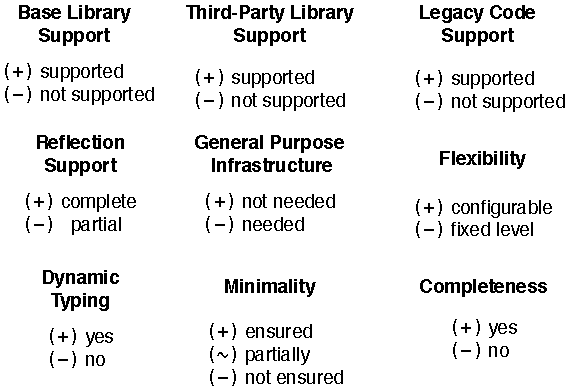
\includegraphics[width=.9\linewidth]{criteria_overview}
 	\caption{Evaluation criteria applied to related work on deployment code unit tailoring techniques}
 	\label{tb:comparison_intro}
 \end{table}

\chapter{Language Virtualization Techniques}

The most related family of work in virtualization are approaches like Xen~\cite{Chis07xen}. Xen is a Virtual Machine Monitor~(VMM) that allows to control and manage \VM in a high performance and resource-managed way. This approach targets the virtualization of full and unmodified operating systems, to facilitate their adoption in industrial/productive environments. They rely on support from the hardware platform, and in some cases from the guest OS, concentrating themselves on performance and production features.

Operating System virtualization technology is characterized by the existence of an \emph{hypervisor}~(named after the Operating System \emph{supervisor} that controls the OS processes\gp{check well that}). The hypervisor is the \VM component that allows one to observe or control the internals of one or many \VMs. A \VM hypervisor gives us, amongst others, the following services:

\begin{description}
\item[Co-location.] Co-location is the ability to have co-existing applications on top of the same virtual machine. With co-location, a single \VM has information about all the applications running on top of itself and can integrate that information in its decision process. Additionally, it gives to co-located applications a cheap communication mechanism as they reside in the same operating system process.
\item[Resource control.] \VMs should control how the different resources of their applications are used. However, state of the art \VMs do only control their consumed memory with the usage of a memory manager. They do not perform in general any control in other kind of resources such as CPU or energy consumption.
\item[Security.] \VMs should control how applications access sensible information such as files and network connections or execute potentially dangerous operations such as system calls.
\item[Application mobility.] As applications are portable, they should be easily migrated between different \VMs also at runtime. Application mobility provides support for resource re-allocation.
\end{description}

High-level languages abstract the developer from the complexities of the underlying machine by running on top of a language \VM. A language \VM provides a language with an execution model closer to its semantics as well as several services such as automatic memory management or cross-cutting optimizations. Language \VMs also provide with portability \ie a program can run on different operating systems and hardware architectures because the \VM abstracts it from the underlying particular details. Although these language \VMs are indeed \emph{Virtual}, state of the art production-ready \VMs do not provide by themselves with the typical advantages of virtualized operating systems such as co-location, resource control, mature security or application mobility support.
With the objective of doing runtime manipulation, we study in the following sections techniques that to our understanding are virtualization-related techniques applied to programming languages runtimes.%We divide theses works in two main topics that are of interest for us in the subject of runtime manipulation. First, we present related work that targets co-location of language runtimes on the same \VM. We continue this section by presenting related work on the subject of runtime control.

\section{\textsc{Class Loaders}}
In Java, classes are loaded dynamically through a class loader~\cite{Lian98a}. A class loader is a first-class entity responsible of loading classes: create their runtime representation, loading their methods and linking their class references. A class loader remembers all classes it loaded, and it is responsible for loading all classes related to  them. Class loaders define namespaces: different class loaders can load classes with the same name. These classes will be isolated in the sense that they will not be visible to the others statically.

Class loaders can be specialized and extended to provide custom behavior. For example, Fong et. al.~\cite{Fong10a} use the class loading mechanism to enforce scoping rules and determine the visibility of names in various region of the program. They allow the user to control untrusted
namespaces and classes and they have defined a language to define security policy. Jensen et. al.~\cite{Jens98a} provide a formalization of the class loader with the means to enforce security. They also use a bytecode verifier on class loading to check if a class' bytecode doesn't try to perform overflow or underflow operations.

In the context of this thesis, we consider the class loader isolation mechanism as it can be used for application co-existence. Different versions of the same application can be loaded by different class loaders and be running at the same time. Class loaders present however a main limitation on the so called \emph{bootstrap class loader}: the literature does not explore the means to load~(and use) different versions of the main runtime classes of the language. Moreover, Java's bootstrap class loader is often implemented natively, and as such, we have no control on it from the language.

Notice additionally that class loaders provide only a load mechanism. Once we loaded several versions of the same application, it does not support the means to manage changes or updates of these applications. In this regard, the OSGI~\cite{OSGI} architecture implementations do often make use of class loaders to load classes into separately isolated components and manage them in a higher level way.

\section{\textsc{Changeboxes}}

Changeboxes~\cite{Denk07c} is a change model designed to encapsulate and scope changes. Its main purpose is to allow several versions of a system to co-exist at runtime \ie the existence in the same environment of different versions of the same classes and methods. In changeboxes, a \emph{changebox} is a first-class entity that encapsulates changes made on the language elements~(\eg classes and methods) and an executable version of the system with its changes applied. The system can contain many changeboxes at the same time, and applications can be scoped to run within different changeboxes. This notion of dynamically scoping an application to a changebox allows one to have co-existing environments~(\eg testing, development, production), increasing the developer's efficiency. Furthermore, it eases application update and migration to new versions, and reduces its update down-time as the application does not have to be stopped to be updated.

A Changeboxes prototype was developed in Smalltalk and its scoping mechanisms were implemented as follows:

\begin{description}
\item[Message send interception.] Message sends can activate different methods, within different changeboxes. A MethodWrapper~\cite{Bran98a} is placed instead of the method that has multiple versions, and it delegates the execution to the method that corresponds to the currently valid changebox.

\item[Class access interception.] Smalltalk resolves class names at compile time, inserting a reference to the given class inside the method's literal array. However, accessing a class should yield different class objects if the changebox contains a different version of it. To resolve this, class accesses affected by a changebox are postponed until runtime, and the code is recompiled in such a way: instead of putting the class inside the literal array, the class is dynamically looked-up from the class table when it is accessed.
\end{description}

Changeboxes model proves sound to update and migrate application and framework classes. However, it has the main drawback of not affecting critical classes in the system. Changeboxes prototype does not work on classes such as \ct{Array} or \ct{CompiledMethod} as the underlying infrastructure~(the VM) restricts the system to the existence of only one of them at the same time. The changes model does not provide neither a solution for this problem, as it focuses on application code update, leaving this as an open problem.

\section{\textsc{Caja\textbackslash Cajita} - Object Capability Languages}

Caja~\cite{Mill08a} is an object-capability language~\cite{Levy84a,Mill03a,Spoo00a} subset of Javascript with the objective of bringing script isolation in Javascript. Caja was thought in the context of the web, where untrusted scripts can be loaded in any webpage and profit from any data available in the webpage. Caja defines a safe Javascript subset that removes elements from the language such as \ct{with} or \ct{eval} because their semantics are strange and in some cases unpredictable. Caja includes Cajita, a subset of Caja without the \ct{this} keyword. Caja is meant for transforming and migrating already existing Javascript code, while Cajita is meant for newly written code.

Caja works with a combination of static and dynamic techniques. First, a static verifier checks and transforms Caja code into sanitized Javascript. This sanitized Javascript contains runtime checks that complements the static verifications. All thee changes are meant to avoid exploits and vulnerabilities from untrusted sources. Caja also adds some new features to the Javascript libraries with support to freeze objects and turn them immutable. 

To allow the safe co-existence of several scripts, Caja removes the Javascript global environment and replaces it by modules. Caja Modules co-exist transparently and can only access each other's data through an explicit and verified interface.
%
%\subsubsection*{\textsc{Worlds}}
%Worlds~\cite{Wart08a} provide a way to control and scope side-effects in Javascript. Side-effects are limited to a first-class environment.

%\subsubsection*{\textsc{Gemstone}}
%Gemstone \cite{Otis91a} provides the concept of class versions. Classes are
%automatically versioned, but existing instances keep the class (shape and
%behavior) of the original definition. Instances can be migrated at any time.
%Gemstone provides (database) transaction semantics, thus state can be rolled
%back should the migration fail.
%Gemstone's class versions extend the usual Smalltalk class evolution mechanism for robustness, 
%large datasets, and domain-specific migration policies. In contrast, ObjectSpaces target general 
%reflective access and bootstrap-like evolutions of code that is critical to the environment.

\section{KaffeOS}

KaffeOS~\cite{Back00a} is a multi-application Java Runtime System centered in application isolation and resource accounting. The KaffeOS runtime allows the isolated co-existence of Java applications so they cannot access each other's data, nor interfere in their execution. To avoid the latter, the KaffeOS \VM accounts the application's consumption of CPU and memory.

KaffeOS adds the process abstraction in the Java language, as in the sense of a process for an operating system. Each KaffeOS process owns a separate memory region~(a process heap) where its object's are allocated. Shared objects reside in special shared memory regions. A \emph{kernel heap} makes a distinction between code that runs in user mode or kernel mode. Regarding process communication, cross-process references become cross-heap references and are handled specially by the \VM. Resources are accounted and controlled at the \VM level for each process, so no process starves other processes.

KaffeOS succeeds to make several Java applications to run side by side taking care on hardware resource consumption in addition of application's data. However, this solution is still limited with respect to base language classes. For example, the class \ct{java.lang.Object} must be shared between different processes to allow their communication.

%J-Kernel \cite{Hawb98a} and Luna \cite{Hawb02a} present a solution similar to ours regarding the memory usage. They are Java solution for isolating object graphs with security purposes. In them, each object graph is called a \emph{protection domain}. All protection domains loaded in a system, and their objects, share the same memory space. 
%
%The J-Kernel enforces the separation between domains by using the Java type system, the inability of the Java language to forge object references, and by providing capability objects\cite{Levy84a,Mill03a,Spoo00a} enabling remote messaging and controlling the communication. This same separation in Luna \cite{Hawb02a} is achieved by the modification of the type system and the addition in the virtual machine of the \emph{remote reference} concept.


\section{JVMTI}
The Java Virtual Machine Tool Interface~(JVMTI)~\cite{JVMPI} is the interface offered by the Java \VM for its manipulation and control. Originally called Java Platform Debugger Architecture~(JPDA) and used in the context of debugging, it was extended to support other use cases such as monitoring and profiling.

JVMTI exposes C functions to manipulate a Java VM~(Figure \ref{fig:jvmti}). The JVMTI client, so called an \emph{Agent}, queries and controls the given JVM through this interface. The manipulated JVM and an agent share the same operating system process. JVMTI agents are meant to be written in C, to be as compact as possible and allow maximal control with minimal intrusion.

\begin{figure}[ht]
\begin{center}
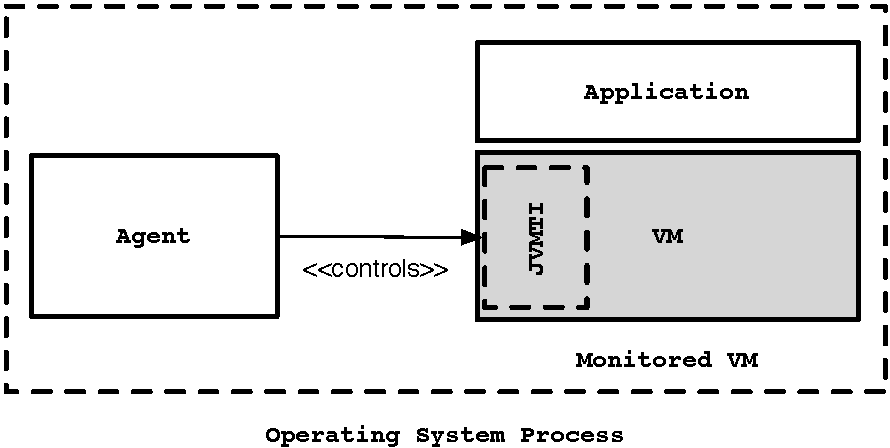
\includegraphics[width=.7\linewidth]{jvmti}
\caption{\textbf{JVMTI Architecture.} An agent controls a JVM though JVMTI. Both share the same operating system process.\label{fig:jvmti}}
\end{center}
\end{figure}

JVMTI provides with introspection and some limited intercession facilities at VM and language level. In particular it provides with memory and heap management, thread control, execution stack manipulation, object and class manipulation and breakpoint support. JVMTI is used mainly with the purpose of debugging, monitoring and analysis, particularly profiling and thread analysis.

In the context of this thesis, we identify in JVMTI's architecture a similarity to a virtualization system. While the Java \VM takes the place of a the virtualized operating system and the agent is its hypervisor and can control.

\section{MVM: a Multi User Virtual Machine}
The Multi-user Virtual Machine~\cite{Czaj03a,Czaj01a} is a general purpose virtual machine for the Java language that allows the co-existence of different applications, potentially from different users. Each application running on top of the MVM is an \emph{isolate} based on the Java Application Isolation API specification~\cite{JSR121}. This Java Application Isolation API defines a uniform mechanism to control the life-cycle of Java applications.

Many isolates co-exist not inteferring each other, as they believe they own their private JVM: the runtime is modified, so state is not shared between them by default. MVM allows several communication mechanisms to securely communicate isolates: from standard mechanisms such as sockets, up to \emph{links}, a low-level isolate-to-isolate mechanism introduced by the Isolate API.

MVM can run unmodified Java applications. Additionally, MVM-aware applications can use the API it provides to control the life-cycle~(\eg creation, suspension, resuming and and termination) and the available resources of other isolates. Notice that differently from JVMTI, this control API is available to the applications running on the JVM and not only to native agents.

%\subsection*{Java Isolates}
%Java Isolates \cite{JSR121} allow multiple applications to run inside the same Java virtual machine.
%Nothing is shared between the different applications. Resources like CPU time, memory are controlled 
%and restricted. Isolates can communicate through channel, since nothing is shared the data are copied. 
%Java Isolates are defined in the Java Specification Request 121, but no commercials Java virtual 
%machine implement the specification.

% =============================================================================

\input{chapter-footer.tex}